\PassOptionsToPackage{unicode=true}{hyperref} % options for packages loaded elsewhere
\PassOptionsToPackage{hyphens}{url}
%
\documentclass[]{article}
\usepackage{lmodern}
\usepackage{amssymb,amsmath}
\usepackage{ifxetex,ifluatex}
\usepackage{fixltx2e} % provides \textsubscript
\ifnum 0\ifxetex 1\fi\ifluatex 1\fi=0 % if pdftex
  \usepackage[T1]{fontenc}
  \usepackage[utf8]{inputenc}
  \usepackage{textcomp} % provides euro and other symbols
\else % if luatex or xelatex
  \usepackage{unicode-math}
  \defaultfontfeatures{Ligatures=TeX,Scale=MatchLowercase}
\fi
% use upquote if available, for straight quotes in verbatim environments
\IfFileExists{upquote.sty}{\usepackage{upquote}}{}
% use microtype if available
\IfFileExists{microtype.sty}{%
\usepackage[]{microtype}
\UseMicrotypeSet[protrusion]{basicmath} % disable protrusion for tt fonts
}{}
\IfFileExists{parskip.sty}{%
\usepackage{parskip}
}{% else
\setlength{\parindent}{0pt}
\setlength{\parskip}{6pt plus 2pt minus 1pt}
}
\usepackage{hyperref}
\hypersetup{
            pdftitle={Extinction risk through climate change in Megafauna},
            pdfauthor={Natalia Villavicencio, Derek Corcoran and Pablo Marquet},
            pdfborder={0 0 0},
            breaklinks=true}
\urlstyle{same}  % don't use monospace font for urls
\usepackage[margin=1in]{geometry}
\usepackage{longtable,booktabs}
% Fix footnotes in tables (requires footnote package)
\IfFileExists{footnote.sty}{\usepackage{footnote}\makesavenoteenv{longtable}}{}
\usepackage{graphicx,grffile}
\makeatletter
\def\maxwidth{\ifdim\Gin@nat@width>\linewidth\linewidth\else\Gin@nat@width\fi}
\def\maxheight{\ifdim\Gin@nat@height>\textheight\textheight\else\Gin@nat@height\fi}
\makeatother
% Scale images if necessary, so that they will not overflow the page
% margins by default, and it is still possible to overwrite the defaults
% using explicit options in \includegraphics[width, height, ...]{}
\setkeys{Gin}{width=\maxwidth,height=\maxheight,keepaspectratio}
\setlength{\emergencystretch}{3em}  % prevent overfull lines
\providecommand{\tightlist}{%
  \setlength{\itemsep}{0pt}\setlength{\parskip}{0pt}}
\setcounter{secnumdepth}{5}
% Redefines (sub)paragraphs to behave more like sections
\ifx\paragraph\undefined\else
\let\oldparagraph\paragraph
\renewcommand{\paragraph}[1]{\oldparagraph{#1}\mbox{}}
\fi
\ifx\subparagraph\undefined\else
\let\oldsubparagraph\subparagraph
\renewcommand{\subparagraph}[1]{\oldsubparagraph{#1}\mbox{}}
\fi

% set default figure placement to htbp
\makeatletter
\def\fps@figure{htbp}
\makeatother

\usepackage[round]{natbib}
\usepackage{booktabs}
\usepackage{longtable}
\usepackage{array}
\usepackage{multirow}
\usepackage{wrapfig}
\usepackage{float}
\usepackage{colortbl}
\usepackage{pdflscape}
\usepackage{tabu}
\usepackage{threeparttable}
\usepackage{threeparttablex}
\usepackage[normalem]{ulem}
\usepackage{makecell}
\usepackage{xcolor}
\usepackage[]{natbib}
\bibliographystyle{plainnat}

\title{Extinction risk through climate change in Megafauna}
\author{Natalia Villavicencio, Derek Corcoran and Pablo Marquet}
\date{}

\begin{document}
\maketitle

\hypertarget{methods}{%
\section{Methods}\label{methods}}

\hypertarget{metrics-of-ectinction}{%
\subsection{Metrics of ectinction}\label{metrics-of-ectinction}}

In order to estimate if the predicted range of a species was low enough for a species to become extinct we estimated the Minimum Viable Area for each species. In order to do that we started by calculating the individual Home Range of a Species as shown in equation \eqref{eq:HomeRange} modified from \citep{lindstedt1986home} to calculate it in \(Km^2\).

\begin{equation}
\begin{aligned}
  HR_{Herb} &= 0.0271 \times M^{1.02} \\
  HR_{Omni} &= 0.034\times M^{0.92} \\
  HR_{Carn} &= 1.37\times M^{1.37}
  \label{eq:HomeRange}
\end{aligned}
\end{equation}

This equation diferienciates between Herbivores, Omnivores and Carnivores, where at the same size Carnivores need much larger range. After that we since we know the area neede by one individual we assume that the Minimum Viable Area (MVA hereafter) is calculated by multipling the Home Range according to equation \eqref{eq:HomeRange},by the Minimum Viable Population (MVP hereafter), as is show in equation \eqref{eq:MVA}, the result of this equation is the \(Km^2\) needed for a species to persist. For MVP we used two estimates from \citep{traill2007minimum}, where it was estimated that the MVP for most vertebrates was 4,169 individuals, but in order to get a more strict estimate we also used the higher estimation of the 95\% confidence interval of 5,129 to make more conservative estimates.

\begin{equation}
  MVA = MVP*HR_{Feed}
  \label{eq:MVA}
\end{equation}

Since the Estimated MVA ranged from 3,947, to 16,426,903 \(Km^2\) we decided to standardize the MVAs as Number of Viable Areas (NVA here after) to make easier to compare between species, the calculation of NVA is shown in equation \eqref{eq:MVA},

\begin{equation}
  NVA = \frac{A}{MVA}
  \label{eq:NVA}
\end{equation}

\hypertarget{species-occurences}{%
\subsection{Species occurences}\label{species-occurences}}

\textbf{{[}{[}Naty{]}{]}}
We rounded the species ocurrences to the nearest decade

\hypertarget{species-distribution-modeling}{%
\subsection{Species Distribution Modeling}\label{species-distribution-modeling}}

We downladed average high and low monthly temperature and average monthly precipitation represented as a difference from present conditions using PaleoView Software \citep{fordham2017paleoview} for the period from 21 kyr BP to the present for South America, using worlclim's version 1.4 as current conditions \citep{hijmans2005very} instead of the newer 2.0 version \citep{fick2017worldclim} since it has 1975 as reference to calculate differences in climate, the same as Paleoview. Then we applied a modified version of the detla method to this layers to consider the changes in sea level \citep{schmatz2015gridded}, using prior works to estimate sealevels \citep[\citet{milne2005modelling}]{fleming1998refining}, and using the gebco bathymetry layers in order to estimate the coastline for each time-slice \citep{weatherall2015new}. After downscaling the layers a 2.5 minute resolution (approximately 5 \(Km^2\)) we used the biovars of the dismo package \citep{Hijman_dismo} to generate bioclimatic layers. The code for the downscaling method can be found at \citep{derek_corcoran_barrios_2020_4016075}

The we used the bioclimatic variables to build the species distribution models following (Phillips et al., 2006; Elith et al., 2011), using the regularization method to avoid overfitting (Allouche et al.,2006; Hastie et al., 2009; Merow et al., 2013). This method allows machine learning algorithm techniques to decide which biolclimatic variables are important to model the distribution of the different species analyzed. The variable selected for each of the species we used in this study can be found in the Supplementary Material section.

\hypertarget{results}{%
\section{Results}\label{results}}

In figure \ref{fig:NVAGraph}, we can see the number of viable areas (NVA hereafter) estimated for each species as a solid line across time, and the lower NVA as a semitransparent area, each time a species NVA drops bellow one (red dashed line),a species is estimated to be extinct. If we look at the estimation, only 2 of the 44 species are predicted to be extinct. The species that should become extinct are Panthera onca mesembrina and Smilodon populator, when we look at the lower estimate interval that number icreases to 3, where the species predicted to become extinct are Panthera onca, Panthera onca mesembrina and Smilodon populator

\begin{figure}
\centering
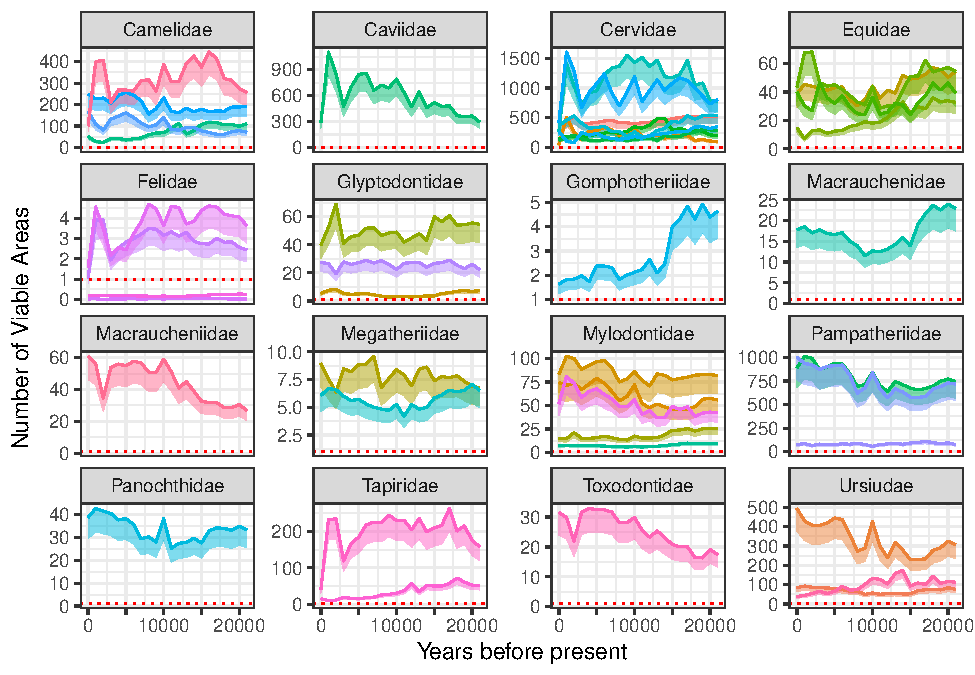
\includegraphics{Manuscript_files/figure-latex/NVAGraph-1.pdf}
\caption{\label{fig:NVAGraph}graph showing the estimation of Number of viable areas for each species and the area showing the lower Estimate of number of viable areas by feeding habits, if a species goes bellow the red dotted line, they are predicted to be extinct}
\end{figure}

\hypertarget{discusion}{%
\section{Discusion}\label{discusion}}

\hypertarget{suplementary-materials}{%
\section{Suplementary materials}\label{suplementary-materials}}

\hypertarget{table-with-all-the-modeled-species}{%
\subsection{Table with all the modeled species}\label{table-with-all-the-modeled-species}}

\begin{longtable}[t]{>{\raggedright\arraybackslash}p{13em}ll>{\raggedright\arraybackslash}p{5em}>{\raggedright\arraybackslash}p{5em}>{\raggedleft\arraybackslash}p{8em}rrr}
\caption{\label{tab:TablaEspecies}Al the modeled species and their mass, estimated Home Range, and the estimated Minimum Viable Area and the Higher interval estimation of the Minimum viable Area}\\
\toprule
Order & Family & Species & State & Feeding & Mass [Kg] & Estimated home range [Km\textasciicircum{}2/ind] & Estimated minimum viable area [Km\textasciicircum{}2] & Higher interval of the minimum viable area [Km\textasciicircum{}2]\\
\midrule
\endfirsthead
\caption[]{\label{tab:TablaEspecies}Al the modeled species and their mass, estimated Home Range, and the estimated Minimum Viable Area and the Higher interval estimation of the Minimum viable Area \textit{(continued)}}\\
\toprule
Order & Family & Species & State & Feeding & Mass [Kg] & Estimated home range [Km\textasciicircum{}2/ind] & Estimated minimum viable area [Km\textasciicircum{}2] & Higher interval of the minimum viable area [Km\textasciicircum{}2]\\
\midrule
\endhead

\endfoot
\bottomrule
\endlastfoot
Artiodactyla & Cervidae & Antifer ultra & Extinct & Herbivore & 114 & 3 & 13,164 & 17,304\\
Carnivora & Ursiudae & Arctotherium tarijense & Extinct & Omnivore & 345 & 7 & 28,488 & 37,447\\
Carnivora & Ursiudae & Arctotherium wingei & Extinct & Omnivore & 217 & 5 & 18,595 & 24,444\\
Artiodactyla & Cervidae & Blastocerus dichotomus & Extant & Herbivore & 114 & 3 & 13,164 & 17,304\\
Pilosa & Mylodontidae & Catonyx chiliense & Extinct & Herbivore & 961 & 30 & 115,806 & 152,227\\
\addlinespace
Pilosa & Mylodontidae & Catonyx cuvieri & Extinct & Herbivore & 1,179 & 37 & 142,658 & 187,524\\
Cingulata & Glyptodontidae & Doedicurus clavicaudatus & Extinct & Herbivore & 1,486 & 47 & 180,639 & 237,450\\
Perissodactyla & Equidae & Equus neogeus & Extinct & Herbivore & 399 & 12 & 47,244 & 62,102\\
Pilosa & Megatheriidae & Eremotherium laurillardi & Extinct & Herbivore & 3,825 & 122 & 473,846 & 622,870\\
Pilosa & Mylodontidae & Glossotherium robustum & Extinct & Herbivore & 1,343 & 42 & 162,926 & 214,166\\
\addlinespace
Cingulata & Glyptodontidae & Glyptodon clavipes & Extinct & Herbivore & 755 & 23 & 90,544 & 119,020\\
Perissodactyla & Equidae & Hippidion devillei & Extinct & Herbivore & 256 & 8 & 30,044 & 39,493\\
Perissodactyla & Equidae & Hippidion principale & Extinct & Herbivore & 408 & 12 & 48,331 & 63,531\\
Perissodactyla & Equidae & Hippidion saldiasi & Extinct & Herbivore & 266 & 8 & 31,242 & 41,067\\
Artiodactyla & Cervidae & Hippocamelus antisensis & Extant & Herbivore & 55 & 2 & 6,259 & 8,228\\
\addlinespace
Artiodactyla & Cervidae & Hippocamelus bisulcus & Extant & Herbivore & 80 & 2 & 9,173 & 12,058\\
Cingulata & Pampatheriidae & Holmesina paulacouti & Extinct & Herbivore & 120 & 4 & 13,871 & 18,234\\
Rodentia & Caviidae & Hydrochoerus hydrochaeris & Extant & Herbivore & 63 & 2 & 7,189 & 9,450\\
Artiodactyla & Camelidae & Lama guanicoe & Extant & Herbivore & 100 & 3 & 11,517 & 15,140\\
Pilosa & Mylodontidae & Lestodon armatus & Extinct & Herbivore & 3,557 & 114 & 440,006 & 578,388\\
\addlinespace
Litopterna & Macrauchenidae & Macrauchenia patachonica & Extinct & Herbivore & 1,044 & 33 & 126,017 & 165,649\\
Artiodactyla & Cervidae & Mazama americana & Extant & Herbivore & 38 & 1 & 4,293 & 5,643\\
Pilosa & Megatheriidae & Megatherium americanum & Extinct & Herbivore & 3,614 & 115 & 447,199 & 587,843\\
Artiodactyla & Cervidae & Morenelaphus brachyceros & Extinct & Herbivore & 50 & 1 & 5,679 & 7,466\\
Cingulata & Panochthidae & Neosclerocalyptus paskoensis & Extinct & Herbivore & 575 & 18 & 68,583 & 90,152\\
\addlinespace
Proboscidea & Gomphotheriidae & Notiomastodon platensis & Extinct & Herbivore & 5,928 & 191 & 740,831 & 973,823\\
Artiodactyla & Cervidae & Odocoileus virginianus & Extant & Herbivore & 85 & 3 & 9,758 & 12,827\\
Artiodactyla & Cervidae & Ozotoceros bezoarticus & Extant & Herbivore & 35 & 1 & 3,947 & 5,189\\
Artiodactyla & Camelidae & Palaeolama major & Extinct & Herbivore & 298 & 9 & 35,080 & 46,112\\
Artiodactyla & Camelidae & Palaeolama weddelli & Extinct & Herbivore & 298 & 9 & 35,080 & 46,112\\
\addlinespace
Cingulata & Pampatheriidae & Pampatherium humboldti & Extinct & Herbivore & 98 & 3 & 11,282 & 14,831\\
Cingulata & Pampatheriidae & Pampatherium typum & Extinct & Herbivore & 200 & 6 & 23,356 & 30,702\\
Cingulata & Glyptodontidae & Panochthus tuberculatus & Extinct & Herbivore & 920 & 29 & 110,769 & 145,605\\
Carnivora & Felidae & Panthera onca & Extant & Carnivore & 76 & 517 & 2,003,637 & 2,633,779\\
Carnivora & Felidae & Panthera onca mesembrina & Extinct & Carnivore & 190 & 1,814 & 7,030,671 & 9,241,813\\
\addlinespace
Carnivora & Felidae & Puma concolor & Extant & Carnivore & 58 & 357 & 1,383,569 & 1,818,700\\
Pilosa & Mylodontidae & Scelidotherium leptocephalum & Extinct & Herbivore & 875 & 27 & 105,245 & 138,344\\
Carnivora & Felidae & Smilodon populator & Extinct & Carnivore & 353 & 4,238 & 16,426,903 & 21,593,155\\
Perissodactyla & Tapiridae & Tapirus bairdi & Extant & Herbivore & 300 & 9 & 35,320 & 46,428\\
Perissodactyla & Tapiridae & Tapirus pinchaque & Extant & Herbivore & 193 & 6 & 22,523 & 29,606\\
\addlinespace
Perissodactyla & Tapiridae & Tapirus terrestris & Extant & Herbivore & 225 & 7 & 26,338 & 34,621\\
Notoungulata & Toxodontidae & Toxodon platensis & Extinct & Herbivore & 2,012 & 63 & 246,067 & 323,455\\
Carnivora & Ursiudae & Tremarctos ornatus & Extant & Herbivore & 200 & 6 & 23,356 & 30,702\\
Artiodactyla & Camelidae & Vicugna vicugna & Extant & Herbivore & 42 & 1 & 4,754 & 6,249\\
Litopterna & Macraucheniidae & Xenorhinotherium bahiense & Extinct & Herbivore & 1,000 & 31 & 120,602 & 158,531\\*
\end{longtable}

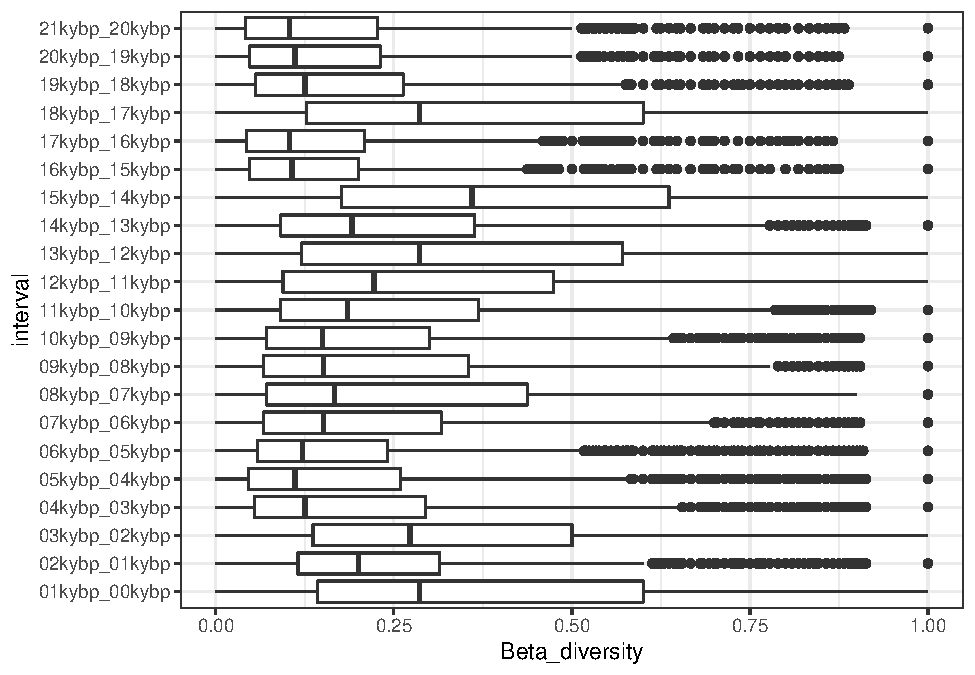
\includegraphics{Manuscript_files/figure-latex/unnamed-chunk-1-1.pdf}

\renewcommand\refname{References}
\bibliography{Biblio.bib}

\end{document}
